% !Mode:: "TeX:UTF-8"
\chapter{绪论}

\section{研究背景及意义}
    随着科技的进步,人类对自然,以及对生命有了更为深刻的认识。从显微镜的发明到DNA双链结构的提出,再到如今的21世纪,伴随着科学研究的深入,人们越来越多地发现,许多重大疾病跟基因相关,如某些癌症、一些先天性的心脏病和肥胖症。Maron\cite{maron2014hypertrophic}等研究发现,大多数肥厚型心肌病、扩张型心肌病的病人中可发现致病基因。对于基因的研究成为了解决或预防这些疾病的关键。在人类的历史上不时出现的大规模传染病,带走了上百万人的生命,对人类的经济甚至文明都产生了巨大的影响。无论是2003年的非典\cite{sars}(SARS),还是2019年底的新型冠状病毒\cite{covid-19}(COVID-19),基因都是研究这些病毒的突破点,解析了其基因的组成和作用,将极大地帮助研究人员研制出对应的抗体。每次病毒的大规模扩散,对所在国家的经济和发展都会带来巨大的损失,因此,基因研究是一项任重而道远的,属于全人类的任务。

    随着生物实验技术的进步,基因测序变得越来越方便和便宜。在美国,已经有公司推出了价格亲民的基因测序产品,人们只需花费数百美元然后在一周之内就可以知道自己的基因序列和表达情况,从而可以提前知道自己有哪些易感基因以及将来容易得哪些疾病,并以此为根据做好预防。在细胞的生物过程中,基因通过转录成信使核糖核酸(mRNA),在不同酶和氨基酸的参与下合成各种各样的蛋白质,这一过程称之为基因的表达。虽然同一生物中的各个体细胞的基因序列是相同的,但不同的细胞仅会在特定的条件下表达特定的极少数基因。mRNA的含量越高,则其代表的基因表达水平越高。所以,研究基因的表达调控是基因组表达分析的重要内容,也有很大的意义,比如,它有助于确认病毒感染和致癌基因,并有助于确认在细胞的各个生命周期内活性基因等。通过高通量基因表达测量技术如微阵列技术(Microarray),可以测得不同mRNA的在细胞体液中的浓度。该数据代表着基因的表达水平,因此被称为基因表达数据。通常情况下,基因表达数据的每一行都有一个相应的基因名字或编号,每一列则代表一个条件或样本。

    在生物信息学中,对基因表达数据的挖掘是研究热点。基因表达数据中含有大量有用的信息。例如,在何种条件下,哪些基因存在类似或相关的表达波动?这些基因都共同参与到了哪些功能或者通路?这些基因受到了哪些调节?如何将隐藏在基因表达数据中的价值挖掘出来并利用,需要大量的计算和研究。数据挖掘领域已经大量成熟的理论和方法供人借鉴,如有监督学习的分类和无监督学习中的聚类。分类技术使得人们更方便地对新产生的数据进行分类,并在医学检测中广泛使用。通过对基因表达数据的聚类分析,可以得到研究人员感兴趣的差异基因。这些基因在不同的实验条件(如样本,时间)下,存在某种一致的表达模式。通过对这些基因的富集或旁路分析,找到这些基因的功能以及相互的调控关系。比如,Eisen\cite{eisen1998cluster}等为了推断基因的新功能,对人类的8600个基因进行了聚类,然后在聚类的结果上利用基因表达谱的相关性进行推断。Tavazoie\cite{tavazoie1999systematic}等使用k均值聚类算法发现了酵母转录调控网络。Tamayo\cite{tamayo1999interpreting} 等利用相似的技术,通过对基因聚类,推断出了新基因的功能和调控网络。 

    然而,基因表达数据有两个主要特点。一,一般而言,基因的数量在几千到几万,而样本或条件的数量只有几十到几百。二,正如前面所诉,基因的表达是条件相关的。基因有可能会在多个条件下表达,也有可能在所有的条件下都没有表达。这些特点使得传统的聚类方法无法胜任,于是就引入了双聚类(Bicluster)的概念,如图\ref{fig:tradiAndBi}所示。不同于传统聚类的全局模式(Global Pattern),双聚类专注于寻找局部模式(Local Pattern),它不要求同一类基因只有在所有实验条件下才具有相似表达,而只要求在部分实验条件下具有相似的表达。找到的基因子集和条件子集就构成了一个双聚类。

    \begin{figure}[htbp]
    \setlength{\subfigcapskip}{-1bp}
    \centering
    \begin{minipage}{.9\textwidth}
    \centering
    \subfigure{}\addtocounter{subfigure}{-2}
    \subfigure{\subfigure[基因方向的传统聚类]{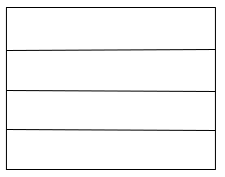
\includegraphics[width=0.29\textwidth]{1}}}
    \hspace{.1em}
    \subfigure{}\addtocounter{subfigure}{-2}
    \subfigure{\subfigure[条件方向的传统聚类]{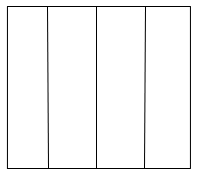
\includegraphics[width=0.25\textwidth]{2}}}
    \hspace{.1em}
    \subfigure{}\addtocounter{subfigure}{-2}
    \subfigure{\subfigure[双聚类]{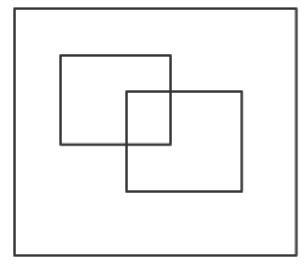
\includegraphics[width=0.25\textwidth]{3}}}
    \end{minipage}
    \vspace{0.2em}
    \caption{传统聚类与双聚类的区别}
    \label{fig:tradiAndBi}
    \end{figure}
    对于传统的聚类方法,其可以从基因或条件方向分别聚类,但是任一条件或基因都将被分配到某一类中去,这与现实中的情况是不符合的。而双聚类允许某些条件或基因不在任一类中出现。双聚类分析已经被证明为NP难问题,因此大部分算法都是通过优化策略来尽可能得找到较优解。同时,因为双聚类的指标之间存在一定程度的负相关,所以双聚类分析可以看作是一种多目标优化问题。在优化算法之中,元启发算法中的群智能算法因其高效和简洁,在学术界和工业界都得到了很大的关注和应用。近年来,针对表达数据高维度、高冗余的特点, 许多群智能优化算法以及多目标优化算法被用于双聚类分析。

\section{相关研究进展}
    从2000年双聚类分析被Cheng和Church引入到基因表达数据挖掘中到现在,双聚类分析经过了近二十年的发展,许多优秀的算法被提出。由于双聚类分析是一个非常困难的问题,这一方向的研究一直在不断地进行着。殷路\cite{yinlu}的研究将双聚类的发展过程大致分为了三个阶段。

    \subsection{早期阶段}
    该阶段的工作主要集中在模型和质量评价上。双聚类(Bicluster)这一单词最早由Hartigan\cite{hartigan1972direct}于1972年提出,但Hartigan只是在行和列两个方向上分别聚类,没有全面地阐述双聚类的概念。直到2000年,Cheng和Church\cite{cc}将双聚类引入到基因表达数据挖掘中,提出了CC算法,并得到了较好的效果。他们提出了MSR(Mean Square Residue,均方残差)用于评价双聚类相似性。MSR越小,则表明行相似性和列相似性越高。该算法先通过不断地删除基因节点和条件节点,找到小于事先给定的MSR阈值$\delta$的双聚类,然后将其作为初始双聚类,在保证MSR不会增大的前提下,不断向其中添加基因节点和条件节点,最终得到一个双聚类结果。如果想要多个结果,算法会把之前找到的双聚类使用随机数覆盖,再重复上述操作,直到获得想要数量的双聚类。随机数的引入,会导致结果不准确,而且无法找到重叠的双聚类。2002年,Yang\cite{floc}等对CC算法进行改进,提出了FLOC算法。算法从多个初始双聚类出发,根据最大增益的原则,来执行基因和条件节点的删除或增加。但并没有解决贪心策略带来的陷入局部最优解的问题。

    有一类双聚类算法使用传统的单向聚类算法以及通过组合和筛选来获得双聚类。Tang\cite{tang2001interrelated}等引入了相互关联的双向聚类(ITWC)算法,该算法结合了在数据矩阵的两个维度上进行单向聚类的结果,从而产生双聚类。 在对数据矩阵的行进行归一化之后,他们计算每行和预定义的稳定模式之间的矢量角度余弦值,以测试行值在列之间的变化是否很大,并删除变化不大的列。 之后,他们使用相关系数作为相似性度量来测量两行或两列之间的线性关系的强度,以执行双向聚类。Getz\cite{getz2000coupled}等提出了耦合双向聚类( Coupled Two-Way Clustering,CTWC)算法。 当CTWC应用于基因表达数据时,其目的是寻找基因的子集和条件的子集,从而单个细胞过程是条件子集上基因子集表达的主要贡献者。Busygin\cite{busygin2002double}等提出了双共轭聚类算法(Double Conjugated Clustering,DCC),该算法在执行时,使用自组织映射(SOM)和角度度量(点积)来计算行和列之间的相似度。

    2002年,Bergmann\cite{isa}等人提出了ISA算法(Iterative Signature Algorithm,迭代签名算法)。ISA并没有使用MSR,而是将双聚类视为转录模块,然后通过对其进行打分,迭代地修改基因集和条件集,直到无法再继续修改。同年,Tanay\cite{tanay2002}等将双聚类定义为在条件(列)的子集之间存在连接反应(jointly respond )的基因(行)子集。 如果基因的表达水平相对于正常水平在该条件下发生显着变化,则该基因被认为对某种条件有反应,并提出了SAMBA(Statistical Algorithm Method For Bicluster Analysis)算法。该算法使用了图论和统计学的知识,将基因表达数据看作一个二分图,一边为基因,一边为条件。通过寻找最大稠密子图的方式来找到基因表达数据中的最大子矩阵,即双聚类。Lazzeroni\cite{plaid}等把基因表达数据看作为背景模型与多个双聚类的叠加,并以此为基础提出了Plaid模型。Ben-dor\cite{ben2002discovering}等将双聚类建模为OPSM(Order Preserving Sub-Matrices),一个在基因表达水平上由连续保持的基因和条件组成的子矩阵,然后使用贪婪启发式算法在基因表达数据中搜索双聚类。出于同样的想法,Liu\cite{liu2003op}等将双聚类定义为OP-Clsuter(Order Preserving Cluster),算法的目标是找到在行方向具有变化趋势一致的双聚类。Murai\cite{murali2002extracting}等将双聚类建模为基因表达的保守模式xMotifs(Conserved Gene Expression Motifs),然后将随机选择的样本作为种子进行扩展,得到满足条件的双聚类,重复该过程,直到所有样本都包含在多个双聚类中。

    Segal\cite{segal2001rich}等利用贝叶斯公式,在基因表达数据上结合先验信息建立了概率模型并称之为RPM (Rich Probabilistic Models)模型。该模型通过期望最大化 EM (Expectation Maximization)算法来确定双聚类。紧接着,Segal\cite{segal2002decomposing}等又在RPM模型的基础上进行扩展,使其能够允许双聚类出现重叠。Wang\cite{wang2002clustering}等提出了pCluster指标来描述基因之间的相似距离,并将找到的双聚类命名为p-Cluster,然后通过枚举和减枝技术来寻找基因表达数据中的双聚类。Sheng\cite{sheng2003biclustering}等基于Gibbs采样算法提出了一种双聚类分析算法。Gibbs采样一定程度上缓解了EM算法容易陷入局部最优的缺点,但是该算法在样本数量远小于基因数量时会有一定的计算困难。

    Califano\cite{califano2000analysis}等提出了一种算法,该算法解决了寻找有效$\delta$-valid模式的问题。他们的目标是找到在各列子集中表现出连贯值但在任何剩余的列中都没有任何连贯性的行组。在对数据进行预处理之后,他们使用模式发现算法来发现行和列候选集是具有统计意义的双聚类(其他候选集被丢弃)。最后,使用贪婪集覆盖算法从统计上重要的模式中选择最佳模式集,该算法将行和列添加到现有模式中,从而使它们成为最大模式。Kluger\cite{kluger2003spectral}等通过假设归一化后的矩阵包含棋盘格结构,使用了一种频谱方法来进行双聚类分析。

    \subsection{壮大阶段}
    该阶段相比早期阶段增加了在元启发式算法和多目标优化算法的研究。由于双聚类问题是NP难问题,通过贪婪或枚举的方法很难高效地得出结果,人们开始使用元启发式算法,如群智能算法来寻找双聚类。2004年,Bleuler\cite{bleuler2004ea}等人设计了一个基因表达数据双聚类分析的进化算法框架。Chakraborty\cite{chakraborty2005biclustering}等同样基于进化算法提出了一种双聚类分析算法。不同于其他算法,该算法没有每一步都执行CC算法,而是只使用CC算法作为初始化步骤。初始种群包括通过K-均值聚类在基因和样本两个维度上结合生成的双聚类种子。紧接着使用进化算法按照适应值寻找容量大且更变化一致的双聚类。
    
    双聚类分析可以看作在均方残差、容量和方差等方向的多目标问题,许多算法使用多目标的方案解决双聚类问题。2006年Mitra\cite{mitra2006multi}提出了多目标进化双聚类的框架,应用经典的非支配排序遗传算法( Non-dominated Sorting Genetic Algorithm-II,NSGA-II)算法,整合局部搜索策略,并提出新的定量度量方法估计双聚类的质量。2007年,Divina\cite{divina2007multi}等提出多目标连续变化双聚类算法 (Sequential Multi objective Biclustering,SMOB)。Coelho\cite{coelho2008multi}等提出了一种基于多目标人工免疫系统的双聚类技术,它能够执行多种群搜索,名为MOM-aiNet。Giraldez\cite{giraldez2007evolutionary}应用最大标准区域(Maximal Standard Area,MSA)作为度量双聚类的标准,并和MSR一起应用到多目标进化算法MOEA中,有效解决了成比例模式的双聚类问题。2013年Brizuela\cite{brizuela2013improving}等提出了一种改进的多目标遗传双聚类算法(Enhanced Multi-objective Genetic Biclustering ,EMOGB)。    

    一些双聚类算法在开发双聚类算法中采用模糊集理论来捕获重叠的双聚类。Tjhi\cite{tjhi2006flexible}等提出了一种灵活的模糊双聚类算法,该算法称为具有特征聚类加权的灵活模糊联合聚类(Flexible Fuzzy Co-clustering with Feature-cluster Weighting,FFCFW),算法将特征聚类加权纳入了公式,允许对象聚类的数量与特征聚类的数量不同。对于由FFCFW生成的每个目标聚类,都采用了一个特征聚类权重方案,以便在特征聚类权重中体现两种类型的聚类之间的关系。这使FFCFW可以更准确地表示模糊共聚体。另外,FFCFW使用迭代的思想进行优化。2007年,Fei X\cite{fei2007gfba}等提出了一种基于遗传算法的模糊双聚类算法GFBA。该算法没有使用二进制串来表示双聚类,而是通过0到1之间的实数值代表相应基因和条件在该双聚类中参与程度。2008年,Han L\cite{han2008fuzzy}等提出了FBMDA(Fuzzy Biclustering for Microarray Data Analysis)算法。该方法结合了Nelder-Mead算法和min-max算法来构造分层结构的双聚类,因此可以表示不同级别的双聚类信息。FBMDA使用多目标优化,可同时优化容量,方差和模糊熵。Nelder-Mead算法用于计算单个目标最优解,而min-max算法用于在多个目标之间进行权衡。

    基于图理论的双聚类在这一阶段也得到了发展。Prelic\cite{prelic2006systematic}等提出了BiMax(Binary inclusion-Maximal)双聚类算法。算法首先根据用户指定的阈值将输入矩阵离散为0和1,基于此二进制矩阵,BiMax可以识别所有最大的双聚类,其中双据类被定义为包含所有1的子矩阵E。inclusion-Maximal表示此双聚类没有完全包含在任何其他双聚类中。基于矩阵E可以推算出双聚类的事实,算法使用增量算法来搜索inclusion-maximal双聚类。由于BiMax与二进制矩阵一起使用,因此它仅适用于检测恒定值的双聚类。2007年,Ahmad\cite{ahmad2007chawk}等将双聚类分析问题转化为加权二部图中最大交叉数减少(最小化)问题,并提出了一种称为cHawk的算法。该算法采用了重心启发式和局部搜索技术。首先,从输入矩阵中构建二分图,然后进行二分图交叉最小化,最终确定双聚类。此方法对矩阵进行重新排序,以使属于同一个双聚类的所有行和列都靠的更近。cHawk能够检测恒定值以及加法模型和重叠的双聚类。

    基于线性代数和矩阵分解理论的双聚类分析方法在这一阶段被提出。Cano\cite{cano2007possibilistic}等人提出了一种基于奇异值分解(SVD)和传统聚类IPC的双聚类方法PSB(Possibilistic Spectral Biclustering)。SVD技术被用来降维以增强聚类过程。首先,算法通过SVD来找到$min(n, m)$个基因表达矩阵的特征向量,其中n和m表示基因表达矩阵的行数和列数,并基于这些特征向量创建几个分区矩阵。然后对代表基因的那些行和代表原始矩阵中的条件的那些列分别执行两种独立的聚类算法。然后将基因聚类和条件聚类进行组合得到候选双聚类,并对其进行后处理以提高双聚类质量。最后,通过输入基因表达矩阵的线性求逆重复整个过程,以便获得表达不足的基因。PSB中使用的聚类算法是Zhang和Leung\cite{ZhangImproved}提出的IPC聚类算法的变体,它混合了可能性和概率方法。MSR用于可能的双聚类和双聚类的筛选,同时在最后一步中也考虑了体积。可能的聚类允许大量的重叠,因此作者还向该过程添加了重叠控件,在该控件中,在添加到结果集中之前检查了双聚类的重叠量。基于nsNMF (non-smooth Non-negative Matrix Factorization)理论,Carmona-Saez\cite{carmona2006biclustering}等提出了的在基因表达数据上确认局部表达模式的双聚类分析方法。
    
    \subsection{当前阶段}
    随着大数据、集成学习、深度学习等技术的发展和普及,许多新型的双聚类分析算法涌现出来。当前阶段除了元启发式算法,双聚类模型和质量评价指标和多目标优化算法之外,增加了以这些新型技术为基础的双聚类研究。基于 Bayesian 理论和双聚类的 Plaid 模型, Zhang\cite{zhang2010bayesian}等提出了 Bayesian Plaid模型。Liu\cite{liu2014gpu}等提出了基于GPU的统一计算设备体系结构(CUDA)的并行 GBC 算法。另外,集成学习因其在聚类方向的广泛应用,也被引入到双聚类分析中。Hanczar\cite{hanczar2010bagging}等应用bagging技术提高CC和Plaid算法的结果质量。基于谱技术,Huang\cite{huang2015spectral}等提出了SCCE(Spectral Co-Clustering Ensemble)双聚类算法。近年来的研究使得神经网络这种深度学习技术取得了突飞猛进的发展,其强大的能力不断地让人们感到惊叹。Sun\cite{sun2013noise}等基于深度学习技术提出了自动解码机(AutoDecoder)算法用来寻找双聚类。陈佳瑜\cite{chenjiayu}结合量子粒子群和FLOC算法,将FLOC算法的输出作为量子粒子群的初始双聚类,取得了不错的效果。殷路\cite{yinlu}提出了基于布谷鸟算法的双聚类算法,并与其他经典的群智能算法进行了比较。

    该阶段有关模式挖掘和关联分析出现了不少的研究工作。Okada\cite{okada2007biclustering}等提出了BiModule算法,该算法允许对输入矩阵进行参数化的多值逐项列出,以使用LCM挖掘算法发现从(闭合)频繁模式中得出的常数双聚类。DeBi\cite{debi}使用MAFIA挖掘算法在二值化矩阵上挖掘的(最大)频繁模式中获得双聚类,并放置关键的后处理原理对其进行调整,以确保其统计意义。Henriques\cite{henriques2014bicpam}等提出的BicPAM通过对输入矩阵执行迭代校正,扩展了先前方法的恒定假设,以找到具有对称,加法和乘法因子的双聚类。BicPAM还引入了为单个元素分配多个离散值的可能性,从而克服了离散化问题,并提供了新的策略来稳健地处理噪声和缺失值。Bellay\cite{bellay2011putting}等使用Apriori算法与其他原理结合使用,以评估所发现的双聚类相对于背景噪声的功能一致性。 Martinez\cite{martinez2007genminer}等提出了GenMiner算法,该算法在输入矩阵中包括外部知识边缘,以从关联规则中导出双聚类,该关联规则将注释(行或列的外部分组)与使用CLOSE关联规则算法从(闭合)频繁模式得出的聚类相关联。BiP算法由Henriques\cite{henriques2015biclustering}等提出,通过依靠耐噪声的关联规则来发现plaid模型,以恢复表观噪声区域,这是由于在双聚类之间重叠区域上存在累积效应。

    2013年,Yan\cite{yan2013biclustering}提出了可以根据不同双聚类类型执行不同搜索策略的BRGCE(Biclustering based on Related Genes and Conditions Extraction)算法。他们根据基因以及条件的稳定性和不同的双聚类类型将层次聚类应用于从输入数据生成的不同数据矩阵。另外,作为预处理步骤,使用James–Stein方法和内核估计原理估计丢失的数据,其中k均值用于获取估计矩阵。Hussain\cite{hussain2016biclustering}等利用明可夫斯基距离和层次聚类提出了SBB(Similarity Based Biclustering)算法。

    基于线性代数的双聚类算法在这一阶段得到了进一步的发展。Yang\cite{yang2010finding}等基于皮尔逊相关系数的子矩阵相关系数SMCS,并提出了BSVD-HC (Biclustering with SVD and Hierarchical Clustering)算法。当双聚类的子矩阵相关系数小于上限$\delta$,则别称为$\delta$-corbicluster。首先,利用SVD获得$C^{(l)}$(一组基本条件)和$R^{(l)}$(一组基本基因)两个矩阵。其次,在将这两个矩阵的行集中之后,通过混合聚类算法,基于聚集层次聚类和使用子矩阵相关性得分作为相异性度量,对它们都进行聚类。这种技术产生的聚类的数目事先未知,因此从这两个矩阵中获得了m和n组聚类。然而,并非每组对都可以是$\delta$-corbicluster,并且执行最后步骤以获得最大包涵的双聚类。最后一步是由Lift算法执行的,该算法受CC算法中提出的节点删除和节点添加阶段的启发,但要根据子矩阵相关性得分。由于聚类算法不会生成互斥的聚类,因此通过此方法获得的双聚类可能会重叠。
    
    2014年,Ahmed\cite{ahmed2014shifting}等提出了一种基于双聚类的移动和缩放相关性(Shifting and Scaling Similarity,SSSim)来评估双聚类的相似性度量,并基于此度量提出了ICS(Intensive Correlation Search)算法。SSSim是使用基线(参考)条件对以及其他条件对的基因局部方法定义的。当评估基因对时,所得分数为从0到1不等,其中值为1表示两个基因都表现出完美的移位和缩放相关性。为了评估双聚类,使用两个输入参数$\tau$和$\alpha$分别考虑基因与部分或完整双聚类之间的相关性。ICS策略迭代地提取不同对基因的相关子空间。这些相关的子空间对应于最大样本集,对于这些样本,基因表达的相关性超过了用户定义的阈值$\tau$。子空间对应于双聚类,该双聚类最初由一对基因形成,并且也被迭代扩展以包括更多基因,直到不能再向双聚类添加任何基因为止。该扩展阶段由第二用户定义的阈值$\alpha$控制。形成初始相关子空间的初始基因对必须由迄今为止不在任何已产生的双聚类的基因形成。但是,这种限制并不能阻止基因在延伸阶段成为多个双聚类的一部分,从而允许双聚类之间的重叠。

    2015年,Chekouo\cite{chekouo2015penalized}等提出了PPM模型(Penalized Plaid Model),该模型主要关注的是阐明双聚类算法背后的相关统计模型。他们发现,许多已知的技术都有潜在的贝叶斯隐患。这一特征促使他们采用贝叶斯框架对双聚类进行建模,并在先前的工作中纳入了两个主要特征:选择双聚类数量的标准和用于解决双聚类之间重叠的惩罚性朴素模型。在此模型中,由于双聚类模型中参数的数量随双聚类的数量呈指数增长,因此采用hard-EM算法用于参数估计。2019年,Singh\cite{singh2019tunable}提出了一种基于图的可调谐双聚类算法(TuBA),该算法基于一种新颖的成对接近度度量,该度量利用数据集的大小来识别肿瘤样本的子集,这些子集相对于其他样本基因以其最高或最低水平共表达。基于共享相似途径的两个基因可能相似的假设,Mandal\cite{mandal2020popbic}等提出了POPBic(Pathway-based Order Preserving Biclustering)算法。POPBic方法的基本原理是在具有大量共同途径的一对基因之间应用最长共同子序列的概念。

\section{论文主要工作}
    因为基因表达数据上双聚类分析的困难性和重要性,过去提出的大量算法都有各自的侧重点。有关基于元启发式的双聚类分析算法,缺少一个较为完整的完整的分析工作。本文以提高双聚类结果的质量指标和生物意义为目标,结合混合元启发式方法和多目标优化方法,对双聚类分析这一问题进行了综合比较研究。本文主要工作如下:
    \begin{itemize}
       \item[1.] {考虑到布谷鸟搜索算法和萤火虫算法的优势互补,本文提出了一种基于布谷鸟搜索和萤火虫算法的混合双聚类分析算法(Cuckoo Search and Firfly Algorithm hybrid Biclustering,CSFAB)。首先,将均方残差,基因容量和样本容量的权重之和作为适应值函数。然后将连续的解转换成比特串来表示双聚类,经过几种混合方式的比较之后,选择了最佳的混合方案。最后在四个常用且数据规模大小不一的基因表达数据集上,通过实验对算法的有效性进行了分析和验证。}

       \item[2.] {双聚类分析其实是多目标优化问题。本文提出了一种多目标细菌觅食算法的双聚类分析算法(Multi-object Bacterial Foraging Algorithm Biclustering,MOBFOB)。算法将均方残差,基因容量和样本容量看作待优化指标,并按照被支配次数对种群排序。以细菌觅食算法为指导,不断地寻找占优的双聚类,并将其保存在外部集合中。最后在四个基因表达数据集上,通过实验对算法的有效性进行了验证。}
       
    \end{itemize}

\section{论文组织结构}
    本文首先对基因表达数据和双聚类分析等相关基础知识进行阐述。然后从单目标优化,混合优化和多目标优化等方面,研究了以群智能算法如布谷鸟搜索算法、萤火虫算法和细菌觅食算法为框架的双聚类算法。最后对本文的工作进行了总结和展望。全文共有五章,本文各章节内容安排如下:

    第一章从生物背景知识出发,讨论了基因研究的重要性以及双聚类的作用和发展现状。双聚类克服了常规聚类与基因表达数据之间的矛盾,能更好的挖掘出有价值的基因子集和条件子集。群智能算法由于其快速且效果更好,在双聚类分析中得到了很广泛地应用。

    第二章先是更具体地讨论的基因表达数据的数学形式,以及双聚类的定义、类型和结构。接着将双聚类算法分为了基于质量评价指标和基于模型两种。然后,对于双聚类结果,讨论了其质量验证指标和生物验证指标。最后分别介绍了本文所关注的群智能算法。

    第三章为了解决普通双聚类算法的质量评价指标不足和生物意义不明显的缺点,本文将布谷鸟算法与萤火虫算法进行了融合,并提出了CSFAB双聚类算法。通过实验,确定了融合的最佳方案,并从质量评价指标和生物评价指标的角度进行了比较分析。

    第四章首先介绍了多目标优化的基本概念,接着将细菌觅食算法按照多目标优化和双聚类的特点进行了改进,包括适应值函数,以及互不支配时的比较规则,并提出了MOBFOB算法。最后根据适应值曲线和生物指标对算法进行了分析。
    
    第五章对全文工作进行了总结和展望。
